% ************************************************************
% Time's Barbed Arrow: Irreversibility, Crypticity, and Stored Information
% Split from main paper: 1/26/09
% jpc: 1/26/09, 2/1/09, 5/15/09

\documentclass[prl,twocolumn,showpacs,superscriptaddress,preprintnumbers,floatfix]{revtex4}

% Packages
\usepackage{ifpdf}
\usepackage{hyperref}
\usepackage{dcolumn}
\usepackage{url}
\usepackage{amsmath}
\usepackage{amssymb}
\usepackage{bm}   % bold math
\usepackage{bbm}   
\usepackage{verbatim}
\usepackage{stmaryrd}
%\usepackage{theorem}
\usepackage{amsthm}

\ifpdf
  \usepackage[pdftex]{graphicx}         % for including graphics
\else
  \usepackage[dvips]{graphicx}
\fi

\theoremstyle{plain}    \newtheorem{Lem}{Lemma}
\theoremstyle{plain}    \newtheorem*{ProLem}{Proof}
\theoremstyle{plain} 	\newtheorem{Cor}{Corollary}
\theoremstyle{plain} 	\newtheorem*{ProCor}{Proof}
\theoremstyle{plain} 	\newtheorem{The}{Theorem}
\theoremstyle{plain} 	\newtheorem*{ProThe}{Proof}
\theoremstyle{plain} 	\newtheorem{Prop}{Proposition}
\theoremstyle{plain} 	\newtheorem*{ProProp}{Proof}
\theoremstyle{plain} 	\newtheorem*{Conj}{Conjecture}
\theoremstyle{plain}	\newtheorem*{Rem}{Remark}
\theoremstyle{plain}	\newtheorem*{Def}{Definition} 
\theoremstyle{plain}	\newtheorem*{Not}{Notation}

% Abbreviations from CMPPSS:

\newcommand{\eM}     {$\epsilon$\protect\nobreakdash-machine}
\newcommand{\eMs}    {$\epsilon$\protect\nobreakdash-machines}
\newcommand{\EM}     {$\epsilon$\protect\nobreakdash-Machine}
\newcommand{\EMs}    {$\epsilon$\protect\nobreakdash-Machines}
\newcommand{\eT}     {$\epsilon$\protect\nobreakdash-transducer}
\newcommand{\eTs}    {$\epsilon$\protect\nobreakdash-transducers}
\newcommand{\ET}     {$\epsilon$\protect\nobreakdash-Transducer}
\newcommand{\ETs}    {$\epsilon$\protect\nobreakdash-Transducers}

% Processes and sequences

\newcommand{\Process}{\mathcal{P}}

\newcommand{\ProbMach}{\Prob_{\mathrm{M}}}
\newcommand{\Lmax}   { {L_{\mathrm{max}}}}
\newcommand{\MeasAlphabet}	{\mathcal{A}}
% Original
%\newcommand{\MeasSymbol}   { {S} }
%\newcommand{\meassymbol}   { {s} }
% New symbol
\newcommand{\MeasSymbol}   { {X} }
\newcommand{\meassymbol}   { {x} }
\newcommand{\BiInfinity}	{ \overleftrightarrow {\MeasSymbol} }
\newcommand{\biinfinity}	{ \overleftrightarrow {\meassymbol} }
\newcommand{\Past}	{ \overleftarrow {\MeasSymbol} }
\newcommand{\past}	{ {\overleftarrow {\meassymbol}} }
\newcommand{\pastprime}	{ {\past}^{\prime}}
\newcommand{\Future}	{ \overrightarrow{\MeasSymbol} }
\newcommand{\future}	{ \overrightarrow{\meassymbol} }
\newcommand{\futureprime}	{ {\future}^{\prime}}
\newcommand{\PastPrime}	{ {\Past}^{\prime}}
\newcommand{\FuturePrime}	{ {\overrightarrow{\meassymbol}}^\prime }
\newcommand{\PastDblPrime}	{ {\overleftarrow{\meassymbol}}^{\prime\prime} }
\newcommand{\FutureDblPrime}	{ {\overrightarrow{\meassymbol}}^{\prime\prime} }
\newcommand{\pastL}	{ {\overleftarrow {\meassymbol}}^L }
\newcommand{\PastL}	{ {\overleftarrow {\MeasSymbol}}^L }
\newcommand{\PastLt}	{ {\overleftarrow {\MeasSymbol}}_t^L }
\newcommand{\PastLLessOne}	{ {\overleftarrow {\MeasSymbol}}^{L-1} }
\newcommand{\futureL}	{ {\overrightarrow{\meassymbol}}^L }
\newcommand{\FutureL}	{ {\overrightarrow{\MeasSymbol}}^L }
\newcommand{\FutureLt}	{ {\overrightarrow{\MeasSymbol}}_t^L }
\newcommand{\FutureLLessOne}	{ {\overrightarrow{\MeasSymbol}}^{L-1} }
\newcommand{\pastLprime}	{ {\overleftarrow {\meassymbol}}^{L^\prime} }
\newcommand{\futureLprime}	{ {\overrightarrow{\meassymbol}}^{L^\prime} }
\newcommand{\AllPasts}	{ { \overleftarrow {\rm {\bf \MeasSymbol}} } }
\newcommand{\AllFutures}	{ \overrightarrow {\rm {\bf \MeasSymbol}} }
\newcommand{\FutureSet}	{ \overrightarrow{\bf \MeasSymbol}}

% Causal states and epsilon-machines
\newcommand{\CausalState}	{ \mathcal{S} }
\newcommand{\CausalStatePrime}	{ {\CausalState}^{\prime}}
\newcommand{\causalstate}	{ \sigma }
\newcommand{\CausalStateSet}	{ \boldsymbol{\CausalState} }
\newcommand{\AlternateState}	{ {\cal R} }
\newcommand{\alternatestate}	{ \rho }
\newcommand{\AlternateStateSet}	{ \boldsymbol{\AlternateState} }
\newcommand{\PrescientState}	{ \widehat{\AlternateState} }
\newcommand{\prescientstate}	{ \widehat{\alternatestate} }
\newcommand{\PrescientStateSet}	{ \boldsymbol{\PrescientState}}
\newcommand{\CausalEquivalence}	{ {\sim}_{\epsilon} }
\newcommand{\CausalEquivalenceNot}	{ {\not \sim}_{\epsilon}}

\newcommand{\NonCausalEquivalence}	{ {\sim}_{\eta} }
\newcommand{\NextObservable}	{ {\overrightarrow {\MeasSymbol}}^1 }
\newcommand{\LastObservable}	{ {\overleftarrow {\MeasSymbol}}^1 }
%\newcommand{\Prob}		{ {\rm P}}
\newcommand{\Prob}		{ {\Pr}}
\newcommand{\ProbAnd}	{ {,\;} }
\newcommand{\LLimit}	{ {L \rightarrow \infty}}
\newcommand{\Cmu}		{ {C_\mu}}
\newcommand{\hmu}		{ {h_\mu}}
\newcommand{\EE}		{ {\bf E}}
\newcommand{\Measurable}{ {\bf \mu}}

% Process Crypticity
\newcommand{\PC}		{\chi}
% Causal Irreversibility
\newcommand{\CI}		{\Xi}
\newcommand{\ReverseMap}	{r}
\newcommand{\ForwardMap}	{f}

% Abbreviations from IB:
% None that aren't already in CMPPSS

% Abbreviations from Extensive Estimation:
\newcommand{\EstCausalState}	{\widehat{\CausalState}}
\newcommand{\estcausalstate}	{\widehat{\causalstate}}
\newcommand{\EstCausalStateSet}	{\boldsymbol{\EstCausalState}}
\newcommand{\EstCausalFunc}	{\widehat{\epsilon}}
\newcommand{\EstCmu}		{\widehat{\Cmu}}
\newcommand{\PastLOne}	{{\Past}^{L+1}}
\newcommand{\pastLOne}	{{\past}^{L+1}}

% Abbreviations from $\epsilon$-Transducers:
\newcommand{\InAlphabet}	{ \mathcal{A}}
\newcommand{\insymbol}		{ a}
\newcommand{\OutAlphabet}	{ \mathcal{B}}
\newcommand{\outsymbol}		{ b}
\newcommand{\InputSimple}	{ X}
\newcommand{\inputsimple}	{ x}
\newcommand{\BottleneckVar}	{\tilde{\InputSimple}}
\newcommand{\bottleneckvar}	{\tilde{\inputsimple}}
\newcommand{\InputSpace}	{ \mathbf{\InputSimple}}
\newcommand{\InputBi}	{ \overleftrightarrow {\InputSimple} }
\newcommand{\inputbi}	{ \overleftrightarrow {\inputsimple} }
\newcommand{\InputPast}	{ \overleftarrow {\InputSimple} }
\newcommand{\inputpast}	{ \overleftarrow {\inputsimple} }
\newcommand{\InputFuture}	{ \overrightarrow {\InputSimple} }
\newcommand{\inputfuture}	{ \overrightarrow {\inputsimple} }
\newcommand{\NextInput}	{ {{\InputFuture}^{1}}}
\newcommand{\NextOutput}	{ {\OutputFuture}^{1}}
\newcommand{\OutputSimple}	{ Y}
\newcommand{\outputsimple}	{ y}
\newcommand{\OutputSpace}	{ \mathbf{\OutputSimple}}
\newcommand{\OutputBi}	{ \overleftrightarrow{\OutputSimple} }
\newcommand{\outputbi}	{ \overleftrightarrow{\outputsimple} }
\newcommand{\OutputPast}	{ \overleftarrow{\OutputSimple} }
\newcommand{\outputpast}	{ \overleftarrow{\outputsimple} }
\newcommand{\OutputFuture}	{ \overrightarrow{\OutputSimple} }
\newcommand{\outputfuture}	{ \overrightarrow{\outputsimple} }
\newcommand{\OutputL}	{ {\OutputFuture}^L}
\newcommand{\outputL}	{ {\outputfuture}^L}
\newcommand{\InputLLessOne}	{ {\InputFuture}^{L-1}}
\newcommand{\inputLlessone}	{ {\inputufutre}^{L-1}}
\newcommand{\OutputPastLLessOne}	{{\OutputPast}^{L-1}_{-1}}
\newcommand{\outputpastLlessone}	{{\outputpast}^{L-1}}
\newcommand{\OutputPastLessOne}	{{\OutputPast}_{-1}}
\newcommand{\outputpastlessone}	{{\outputpast}_{-1}}
\newcommand{\OutputPastL}	{{\OutputPast}^{L}}
\newcommand{\OutputLPlusOne}	{ {\OutputFuture}^{L+1}}
\newcommand{\outputLplusone}	{ {\outputfutre}^{L+1}}
\newcommand{\InputPastL}	{{\InputPast}^{L}}
\newcommand{\inputpastL}	{{\inputpast}^{L}}
\newcommand{\JointPast}	{{(\InputPast,\OutputPast)}}
\newcommand{\jointpast}	{{(\inputpast,\outputpast)}}
\newcommand{\jointpastone}	{{(\inputpast_1,\outputpast_1)}}
\newcommand{\jointpasttwo}	{{(\inputpast_2,\outputpast_2)}}
\newcommand{\jointpastprime} {{({\inputpast}^{\prime},{\outputpast}^{\prime})}}
\newcommand{\NextJoint}	{{(\NextInput,\NextOutput)}}
\newcommand{\nextjoint}	{{(\insymbol,\outsymbol)}}
\newcommand{\AllInputPasts}	{ { \overleftarrow {\rm \InputSpace}}}
\newcommand{\AllOutputPasts}	{ {\overleftarrow {\rm \OutputSpace}}}
\newcommand{\DetCausalState}	{ {{\cal S}_D }}
\newcommand{\detcausalstate}	{ {{\sigma}_D} }
\newcommand{\DetCausalStateSet}	{ \boldsymbol{{\CausalState}_D}}
\newcommand{\DetCausalEquivalence}	{ {\sim}_{{\epsilon}_{D}}}
\newcommand{\PrescientEquivalence}	{ {\sim}_{\widehat{\eta}}}
\newcommand{\FeedbackCausalState}	{ \mathcal{F}}
\newcommand{\feedbackcausalstate}	{ \phi}
\newcommand{\FeedbackCausalStateSet}	{ \mathbf{\FeedbackCausalState}}
\newcommand{\JointCausalState}		{ \mathcal{J}}
\newcommand{\JointCausalStateSet}	{ \mathbf{\JointCausalState}}
\newcommand{\UtilityFunctional}	{ {\mathcal{L}}}
\newcommand{\NatureState}	{ {\Omega}}
\newcommand{\naturestate}	{ {\omega}}
\newcommand{\NatureStateSpace}	{ {\mathbf{\NatureState}}}
\newcommand{\AnAction}	{ {A}}
\newcommand{\anaction}	{ {a}}
\newcommand{\ActionSpace}	{ {\mathbf{\AnAction}}}

% Abbreviations from RURO:
\newcommand{\InfoGain}[2] { \mathcal{D} \left( {#1} || {#2} \right) }

% Abbreviations from Upper Bound:
\newcommand{\lcm}	{{\rm lcm}}
% Double-check that this isn't in the math set already!

% Abbreviations from Emergence in Space
\newcommand{\ProcessAlphabet}	{\MeasAlphabet}
\newcommand{\ProbEst}			{ {\widehat{\Prob}_N}}
\newcommand{\STRegion}			{ {\mathrm K}}
\newcommand{\STRegionVariable}		{ K}
\newcommand{\stregionvariable}		{ k}
\newcommand{\GlobalPast}		{ \overleftarrow{G}} 
\newcommand{\globalpast}		{ \overleftarrow{g}} 
\newcommand{\GlobalFuture}		{ \overrightarrow{G}}
\newcommand{\globalfuture}		{ \overrightarrow{g}}
\newcommand{\GlobalState}		{ \mathcal{G}}
\newcommand{\globalstate}		{ \gamma}
\newcommand{\GlobalStateSet}		{ {\mathbf \GlobalState}}
\newcommand{\LocalPast}			{ \overleftarrow{L}} 
\newcommand{\localpast}			{ \overleftarrow{l}}
\newcommand{\AllLocalPasts}		{ \mathbf{\LocalPast}}
\newcommand{\LocalPastRegion}		{ \overleftarrow{\mathrm L}}
\newcommand{\LocalFuture}		{ \overrightarrow{L}}
\newcommand{\localfuture}		{ \overrightarrow{l}}
\newcommand{\LocalFutureRegion}		{ \overrightarrow{\mathrm L}}
\newcommand{\LocalState}		{ \mathcal{L}}
\newcommand{\localstate}		{ \lambda}
\newcommand{\LocalStateSet}		{ {\mathbf \LocalState}}
\newcommand{\PatchPast}			{ \overleftarrow{P}}
\newcommand{\patchpast}			{ \overleftarrow{p}}
\newcommand{\PatchPastRegion}		{ \overleftarrow{\mathrm P}}
\newcommand{\PatchFuture}		{ \overrightarrow{P}}
\newcommand{\patchfuture}		{ \overrightarrow{p}}
\newcommand{\PatchFutureRegion}		{ \overrightarrow{\mathrm P}}
\newcommand{\PatchState}		{ \mathcal{P}}
\newcommand{\patchstate}		{ \pi}
\newcommand{\PatchStateSet}		{ {\mathbf \PatchState}}
\newcommand{\LocalStatesInPatch}	{\vec{\LocalState}}
\newcommand{\localstatesinpatch}	{\vec{\localstate}}
\newcommand{\PointInstantX}		{ {\mathbf x}}
% Galles's original LaTeX for the cond. indep. symbol follows:
\newcommand{\compos}{\mbox{$~\underline{~\parallel~}~$}}
\newcommand{\ncompos}{\not\hspace{-.15in}\compos}
\newcommand{\indep}			{ \rotatebox{90}{$\models$}}
\newcommand{\nindep}	{\not\hspace{-.05in}\indep}
\newcommand{\LocalEE}	{{\EE}^{loc}}
\newcommand{\EEDensity}	{\overline{\LocalEE}}
\newcommand{\LocalCmu}	{{\Cmu}^{loc}}
\newcommand{\CmuDensity}	{\overline{\LocalCmu}}

%%%%%%%%%%% added by sasa
\newcommand{\FinPast}[1]	{ \overleftarrow {\MeasSymbol} \stackrel{{#1}}{}}
\newcommand{\finpast}[1]  	{ \overleftarrow {\meassymbol}  \stackrel{{#1}}{}}
\newcommand{\FinFuture}[1]		{ \overrightarrow{\MeasSymbol} \stackrel{{#1}}{}}
\newcommand{\finfuture}[1]		{ \overrightarrow{\meassymbol} \stackrel{{#1}}{}}

\newcommand{\Partition}	{ \AlternateState }
\newcommand{\partitionstate}	{ \alternatestate }
\newcommand{\PartitionSet}	{ \AlternateStateSet }
\newcommand{\Fdet}   { F_{\rm det} }

\newcommand{\Dkl}[2] { D_{\rm KL} \left( {#1} || {#2} \right) }

\newcommand{\Period}	{p}

% To take into account time direction
\newcommand{\FutureProcess}	{ {\Process}^+ }
\newcommand{\PastProcess}	{ {\Process}^- }
\newcommand{\FutureCausalState}	{ {\CausalState}^+ }
\newcommand{\futurecausalstate}	{ \sigma^+ }
\newcommand{\altfuturecausalstate}	{ \sigma^{+\prime} }
\newcommand{\PastCausalState}	{ {\CausalState}^- }
\newcommand{\pastcausalstate}	{ \sigma^- }
\newcommand{\BiCausalState}		{ {\CausalState}^{\pm} }
\newcommand{\bicausalstate}		{ {\sigma}^{\pm} }
\newcommand{\FutureCausalStateSet}	{ {\CausalStateSet}^+ }
\newcommand{\PastCausalStateSet}	{ {\CausalStateSet}^- }
\newcommand{\BiCausalStateSet}	{ {\CausalStateSet}^{\pm} }
\newcommand{\eMachine}	{ M }
\newcommand{\FutureEM}	{ {\eMachine}^+ }
\newcommand{\PastEM}	{ {\eMachine}^- }
\newcommand{\BiEM}		{ {\eMachine}^{\pm} }
\newcommand{\BiEquiv}	{ {\sim}^{\pm} }
\newcommand{\Futurehmu}	{ h_\mu^+ }
\newcommand{\Pasthmu}	{ h_\mu^- }
\newcommand{\FutureCmu}	{ C_\mu^+ }
\newcommand{\PastCmu}	{ C_\mu^- }
\newcommand{\BiCmu}		{ C_\mu^{\pm} }
\newcommand{\FutureEps}	{ \epsilon^+ }
\newcommand{\PastEps}	{ \epsilon^- }
\newcommand{\BiEps}	{ \epsilon^{\pm} }
\newcommand{\FutureSim}	{ \sim^+ }
\newcommand{\PastSim}	{ \sim^- }
% Used arrows for awhile, more or less confusing?
%\newcommand{\FutureCausalState}	{ \overrightarrow{\CausalState} }
%\newcommand{\PastCausalState}	{ \overleftarrow{\CausalState} }
%\newcommand{\eMachine}	{ M }
%\newcommand{\FutureEM}	{ \overrightarrow{\eMachine} }
%\newcommand{\PastEM}	{ \overleftarrow{\eMachine} }
%\newcommand{\FutureCmu}	{ \overrightarrow{\Cmu} }
%\newcommand{\PastCmu}	{ \overleftarrow{\Cmu} }


\addtolength{\abovedisplayskip}{-.05in}
\addtolength{\belowdisplayskip}{-.05in}
\addtolength{\dbltextfloatsep}{-.10in}
\addtolength{\abovecaptionskip}{-.10in}
\addtolength{\belowcaptionskip}{-.10in}
\parskip 0pt

\begin{document}

\title{Time's Barbed Arrow:\\
Irreversibility, Crypticity, and Stored Information}

\author{James P. Crutchfield}
\email{chaos@cse.ucdavis.edu}
\affiliation{Complexity Sciences Center and Physics Department,
University of California at Davis, One Shields Avenue, Davis, CA 95616}
\affiliation{Santa Fe Institute, 1399 Hyde Park Road, Santa Fe, NM 87501}

\author{Christopher J. Ellison}
\email{cellison@cse.ucdavis.edu}
\affiliation{Complexity Sciences Center and Physics Department,
University of California at Davis, One Shields Avenue, Davis, CA 95616}

\author{John R. Mahoney}
\email{jrmahoney@ucdavis.edu}
\affiliation{Complexity Sciences Center and Physics Department,
University of California at Davis, One Shields Avenue, Davis, CA 95616}

\date{\today}

\bibliographystyle{unsrt}

% ************************* ABSTRACT *************************
\begin{abstract}
We show why the amount of information communicated between the past and
future---the \emph{excess entropy}---is not in general the amount of
information stored in the present---the \emph{statistical complexity}.
This is a puzzle, and a long-standing one, since the former describes
observed behavior, while optimal prediction requires the latter. We
present a closed-form expression for the excess entropy in terms of
optimal causal predictors and retrodictors---both \eMs\ of computational
mechanics. This leads us to two new system invariants:
\textit{causal irreversibility}---the asymmetry between the causal
representations---and \textit{crypticity}---the degree to which a process
hides its state information.
\end{abstract}

\pacs{
02.50.-r  %  Probability theory, stochastic processes, and statistics
89.70.Cf  %  Entropy and other measures of information
05.45.Tp  %  Time series analysis
02.50.Ey  %  Stochastic processes 
% 02.50.Ga  %  Markov processes 
% 05.20.-y  %  Classical statistical mechanics
% 05.45.-a  %  Nonlinear dynamics and nonlinear dynamical systems
% 89.75.Kd  %  Complex Systems: Patterns 
}
%
\preprint{Santa Fe Institute Working Paper 09-02-002}
\preprint{arxiv.org:0902.1209 [cond-mat.stat-mech]}

\maketitle

% ****************************************************************

%\tableofcontents

%  ************************* INTRODUCTION *************************

Constructing a theory can be viewed as our attempt to extract from measurements
a system's hidden organization. This suggests a parallel with decryption whose
goal is to reveal internal correlations within an encrypted data
stream~\cite{Shan49a}. The hidden message is revealed only to a recipient with
the correct codebook. This is essentially the circumstance a scientist faces
when building a model from measurements: What are the hidden states and dynamic
in the observed data?

In this view, the now-long history in nonlinear dynamics of reconstructing 
models from time series~\cite{Kant06a,Spro03a} is cast as a \emph{self-decoding}
problem, where the information used to build a model is only that available in
the observed process. That is, no ``side-band'' communication, prior knowledge,
or disciplinary assumptions are allowed. Nature speaks for herself only through
the data she willingly gives up.

Here, we show that the parallel is more than metaphor: building a model
corresponds directly to decrypting the hidden state information in measurements.
The results show why predicting and modeling are, at one and the same time,
distinct and intimately related. Along the way, we clarify the role and types
of information in prediction and modeling. We show how to measure the degree
of hidden information and identify a new kind of statistical irreversibility.

A process $\Prob(\Past,\Future)$ is a \emph{communication channel} with
a fixed input distribution $\Prob(\Past)$:
It transmits information from the \emph{past}
$\Past = \ldots \MeasSymbol_{-3} \MeasSymbol_{-2} \MeasSymbol_{-1}$ to the
\emph{future} $\Future = \MeasSymbol_0 \MeasSymbol_1 \MeasSymbol_2 \ldots$
by storing it in the present. Here, $\MeasSymbol_t$ is the discrete random
variable for the measurement outcome at time $t$, such as the observed
$z$-component of a spin or the symbolic dynamics of a chaotic system.

Our goal is also simply stated: We wish to
predict the future using information from the past. At root, a prediction is
probabilistic, specified by a distribution of possible futures $\Future$
given a particular past $\past$: $\Prob(\Future|\past)$. At a minimum, a
good predictor needs to capture \emph{all} of the information $I$ shared
between past and future: $\EE = I[\Past;\Future]$---the process's
\emph{excess entropy}~\cite[and references therein]{Crut01a}.

Consider now the goal of modeling: build a representation that not only
allows good prediction, but also expresses the mechanisms that produce a
system's behavior. To build a model of a process,
computational mechanics~\cite{CompMechMerge} introduced an equivalence
relation $\past \sim \past^\prime$ to group all histories that give rise to the
same prediction---resulting in a map from pasts to the \emph{causal states}:
$\epsilon(\past) =
  \{ \past^\prime: \Prob(\Future|\past) = \Prob(\Future|\past^\prime) \}$. 
A process's causal states, $\CausalStateSet = \Prob(\Past,\Future) / \sim$,
partition the space $\AllPasts$ of pasts into sets that are predictively
equivalent. The set of causal states can be discrete, fractal, or continuous.
%\footnote{A process's causal states consist of both transient and recurrent
%states. To simplify the presentation, we henceforth refer \emph{only} to
%recurrent causal states that are discrete.}.
State-to-state transitions are
denoted by matrices $T_{\CausalState \CausalState^\prime}^{(x)}$ whose elements
give the probability of transitioning from one state $\CausalState$ to the
next $\CausalState^\prime$ on seeing measurement value $\meassymbol$. The
resulting model, consisting of the
causal states and transitions, is called the process's \emph{\eM}.
 
Causal states have the Markovian property that they render the past and future
statistically independent; they \emph{shield} the future from the past~%
\cite{CompMechMerge}:
$\Prob(\Past,\Future|\CausalState)
  = \Prob(\Past|\CausalState) \Prob(\Future|\CausalState)$.
In this way, the causal states give a structural decomposition of
the process into conditionally independent modules.
Moreover, they are optimally predictive~\cite{CompMechMerge} in the sense that
knowing which causal state a process is in is just as good as having the
entire past: $\Prob(\Future|\CausalState) = \Prob(\Future|\Past)$. In other
words, causal shielding is equivalent to the fact~\cite{CompMechMerge} that the
causal states capture all of the information shared between past and future:
$I[\CausalState;\Future] = \EE$.

Naturally, there can be alternative models; denote their states
$\AlternateStateSet$. Consider the subset of these that are optimally
predictive---those for which $I[\PrescientState;\Future] = \EE$, where we
denoted their states as $\PrescientStateSet$. Out of all optimally predictive
models, the \eM\ captures the minimal amount of information that a process must
store in order to communicate all of the excess entropy from the past to the
future. This is the \emph{statistical complexity}~\cite{CompMechMerge}: 
$\Cmu \equiv H[\CausalState] \leq H[\PrescientState]$, where $\mu$ reminds 
us of the dependence on the dynamical system's underlying invariant measure. 
In short, $\EE$ is the effective information transmission capacity of the
process, viewed as a channel, and $\Cmu$ is the sophistication of that channel.

In addition to $\EE$ and $\Cmu$, another key (and historically prior)
invariant for dynamical systems and stochastic processes is the entropy rate
$\hmu$---a process's degree of intrinsic randomness~\cite{Shan48a}. Importantly,
the \eM\ immediately gives two of these three important invariants: a process's
rate ($\hmu$) of producing information and the amount ($\Cmu$) of historical
information stored in doing so.

To date, $\EE$ cannot be as directly calculated as the entropy rate and the 
statistical complexity. One practical consequence is that it is difficult to
know when one has obtained a good estimate of $\EE$. These are truly
unfortunate, since excess entropy, and related mutual information quantities,
are widely used diagnostics
for processes, having been applied to detect the presence of organization in
dynamical systems~\cite{Fras86a,Casd91a,Spro03a,Kant06a}, in spin systems~%
\cite{Crut97a,Erb04a}, in neurobiological systems~\cite{Tono94a,Bial00a}, and
even in language, to mention only a few applications. For example, in natural
language the excess entropy appears to diverge with string length $L$ as
$\EE \propto L^{1/2}$, reflecting the long-range and strongly nonergodic
organization necessary for human communication~\cite{Ebel94c,Debo08a}.

This state of affairs has been a major impediment to understanding the
relationships between modeling and predicting and, more concretely, the
relationships between (and even the interpretation of) a process's basic
invariants---$\hmu$, $\Cmu$, and $\EE$
\footnote{Compared to other information-theoretic measures of organization,
$\EE$ is the most general, being the ``all-point'' mutual information
\cite{Crut01a}.
Of the alternative measures of stored information, $\Cmu$ is the most
general since the \eM, from which it is derived, is a minimal
sufficient statistic for a process \cite{CompMechMerge}.}.
Here, we clarify these issues by deriving explicit expressions for $\EE$ in
terms of the \eM\ and $\Cmu$, providing a unified information-theoretic
analysis of stationary processes.

The above development of \eMs\ concerns using the past to predict the future.
But what about the opposite, using the future to retrodict the past?
Usually, one thinks of successive measurements occurring as time
increases. Now, consider scanning the measurement variables not in
the forward time direction, but in the reverse time direction. The 
computational mechanics formalism is essentially unchanged, though its meaning 
and notation need to be augmented.

With this in mind, the previous mapping from pasts to causal states is
denoted $\FutureEps$ and it gave, what we will call, the
\emph{predictive} causal states
$\FutureCausalStateSet$. When scanning in the reverse direction, we
have a new relation, $\future \PastSim \future^\prime$, which groups futures
that are equivalent for the purpose of retrodicting the past:
$\PastEps(\future) =
  \{ \future^\prime: \Prob(\Past|\future) = \Prob(\Past|\future^\prime) \}$.
It gives the \emph{retrodictive} causal states
$\PastCausalStateSet = \Prob(\Past,\Future) / \PastSim$.
And, not surprisingly, we must also distinguish a process's forward-scan
\eM\ $\FutureEM$ from its reverse-scan \eM\ $\PastEM$. They assign
corresponding entropy rates, $\Futurehmu$ and $\Pasthmu$, and
statistical complexities, $\FutureCmu \equiv H[\FutureCausalState]$
and $\PastCmu \equiv H[\PastCausalState]$,
respectively, to the process.

Now we are in a position to ask some questions. Perhaps the most obvious is,
In which time direction is a process most predictable? The answer is that a
stationary process is equally predictable in either~\cite{CompMechMerge}:
$\Pasthmu = \Futurehmu$. Somewhat surprisingly, though, the effort involved
in doing so need not be the same~\cite{Crut91bc}: 
$\PastCmu \neq \FutureCmu$.
Naturally, $\EE$ is mute on this score, since the mutual information $I$ is
symmetric in its variables~\cite{Crut01a}.

The relationship between predicting and retrodicting a process, and ultimately
$\EE$'s role, requires teasing out how the states of the forward and reverse
\eMs\ capture information from the past and the future. To do this we must
analyze a four-variable mutual information:
$I[\Past;\Future;\FutureCausalState;\PastCausalState]$.
A large number of expansions of this quantity are possible. A systematic
development follows from Ref.~\cite{Yeun91a} which showed that Shannon entropy
$H[\cdot]$ and mutual information $I[\cdot;\cdot]$ form a signed measure over
the space of events.

\begin{figure}[th]
\begin{center}
\resizebox{!}{1.6in}{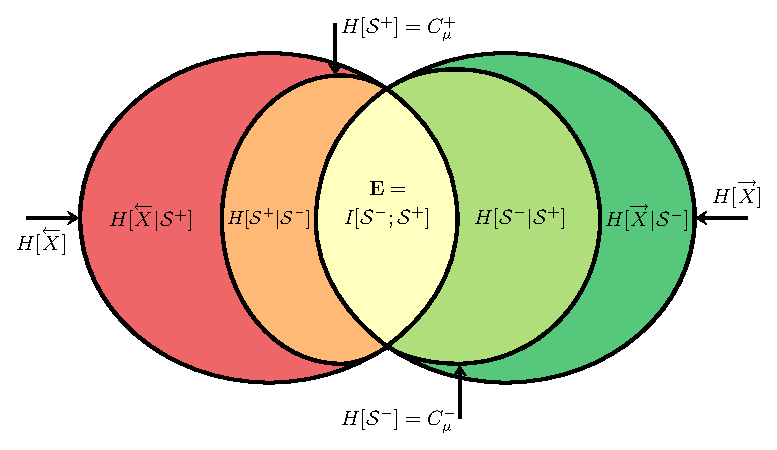
\includegraphics{IDiagramEM}}
\end{center}
\caption{
  \EM\ information diagram for stationary stochastic processes. A schematic,
  the diagram only shows the set-theoretic relationships.
  }
\label{fig:eMIDiagram}
\end{figure}

Using an information measure expansion, it turns out there are 15 possible
relationships to consider for
$I[\Past;\Future;\FutureCausalState;\PastCausalState]$. Fortunately,
this greatly simplifies in the case of using an \eM\ to represent
a process: There are only five relationships.
%\cite{Crut08b}.
(See Fig.~\ref{fig:eMIDiagram}.)
Simplified in this way, we are left with our main results which, due to the
preceding effort, are particularly transparent.
\begin{The}
%\cite{Crut08b}
Excess entropy is the mutual information between the predictive
and retrodictive causal states:
\vspace{-0.1in}
\begin{equation}
\EE = I[\FutureCausalState;\PastCausalState] ~.
\end{equation}
\label{EasCausalMI}
\end{The}
\vspace{-0.3in}
\noindent
This is obtained via a simultaneous reduction of the four-variable mutual
information into
$I[\Past;\Future]$ and $I[\FutureCausalState;\PastCausalState]$.
Notably, the process's channel 
utilization $\EE = I[\Past;\Future]$ between
the past and future is the same as the utilization between the forward and 
reverse \eM\ states. Moreover,
the \emph{predictive statistical complexity} is given by
$\FutureCmu = \EE + H[\FutureCausalState|\PastCausalState]$
and the \emph{retrodictive statistical complexity} by
$\PastCmu = \EE + H[\PastCausalState|\FutureCausalState]$.

Theorem~\ref{EasCausalMI} and the companion results give an explicit
connection between
a process's excess entropy and its causal structure---its \eMs. More generally,
the relationships directly tie mutual information measures of observed
sequences to a process's structure. They will allow us to probe the properties
that control how closely observed statistics reflect a process's
hidden structure; that is, the degree to which observed behavior directly
reflects internal state information.

At this point we have two separate \eMs, one for predicting and one for
retrodicting. We will now show that one can do better, by combining causal
information from the past and future. Consider scanning a realization,
$\biinfinity = \past_t \future_t$, of the process in the forward
direction---seeing histories $\past_t$ and noting the series of causal states
$\FutureCausalState_t = \FutureEps(\past_t)$. Now change direction. What
reverse causal state is one in? This is
$\PastCausalState_t = \PastEps(\future_t)$. We describe the action of changing
scan direction with the \emph{bidirectional machine} $\BiEM$, which is given
by the equivalence relation $\BiEquiv$:
\begin{equation*}
\BiEps(\biinfinity) = \{ (\pastprime,\futureprime):
  	\pastprime \in \FutureEps(\past) ~\mathrm{and}~
	\futureprime \in \PastEps(\future) \}
\end{equation*}
and has causal states $\BiCausalStateSet = \Prob(\Past,\Future) /
\BiEquiv \subset \FutureCausalStateSet \times \PastCausalStateSet$.
That is, the bidirectional causal state the process is in at time $t$ is
$\BiCausalState_t = (\FutureEps(\past_t),\PastEps(\future_t))$.
The amount of stored information needed to optimally predict \emph{and}
retrodict a process is $\BiEM$'s statistical complexity:
$\BiCmu \equiv H[\BiCausalState] = H[\FutureCausalState,\PastCausalState]$.

From the immediately preceding results we obtain the following simple, useful
relationship: $\EE = \FutureCmu + \PastCmu - \BiCmu$.
This suggests a wholly new interpretation of the excess entropy---in
addition to the original three reviewed in Ref.~\cite{Crut01a}: $\EE$ is
exactly the difference between these statistical complexities. Moreover,
only when $\EE = 0$ does $\BiCmu = \FutureCmu + \PastCmu$.
The bidirectional machine is also efficient:
$\BiCmu \leq \FutureCmu + \PastCmu$.
And we have the bounds:
$\FutureCmu \leq \BiCmu$ and $\PastCmu \leq \BiCmu$.
These inequalities express the compactness of the bidirectional
machine in contrast to the pair of directional \eMs. This 
efficiency of representation is due to the redundancy in the 
predictive and retrodictive causal states.

We noted above that predicting and retrodicting may require different amounts
of information storage ($\FutureCmu \neq \PastCmu$). It is helpful to use
\emph{causal irreversibility} to measure this asymmetry~\cite{Crut91bc}:
$\CI \equiv \FutureCmu - \PastCmu$. With the above results, however, we see that
$\CI = H[\FutureCausalState|\PastCausalState] -
H[\PastCausalState|\FutureCausalState]$.
Note that irreversibility is also not controlled by $\EE$, as the
latter is scan-symmetric.

The relationship between excess entropy and statistical complexity established
by Thm.~\ref{EasCausalMI} indicates that there are fundamental limitations on
the amount of a process's stored information ($\BiCmu$) directly present in
observations ($\EE$). We now introduce a measure of this: A process's
\emph{crypticity} is
$\PC \equiv H[\FutureCausalState|\PastCausalState]
+ H[\PastCausalState|\FutureCausalState]$.
This is the distance between a process's forward and reverse \eMs\ and
expresses, most explicitly, the difference between prediction and modeling.
To see this, we need the following connection.
\begin{Cor}
$\BiEM$'s statistical complexity is:
\vspace{-0.07in}
\begin{equation}
\BiCmu = \EE + \PC ~.
\end{equation}
\end{Cor}
\vspace{-0.07in}
\noindent
Referring to $\PC$ as crypticity derives from this result: It
is the amount of internal state information ($\BiCmu$) not directly
present in the observed sequence ($\EE$). That is, a process hides
$\PC$ bits of information.

If crypticity is low ($\PC \approx 0$), then much of the stored
information is present in observed behavior: $\EE \approx \BiCmu$. However,
when a process's crypticity is high, $\PC \approx \BiCmu$, then little of
it's structural information is directly present in observations. Moreover,
there are truly cryptic processes ($\EE \approx 0$) that are highly
structured ($\BiCmu \gg 0$). Little or nothing can be learned from measurements
about such processes's hidden organization.

\begin{figure}[th]
\begin{center}
\resizebox{!}{3.3in}{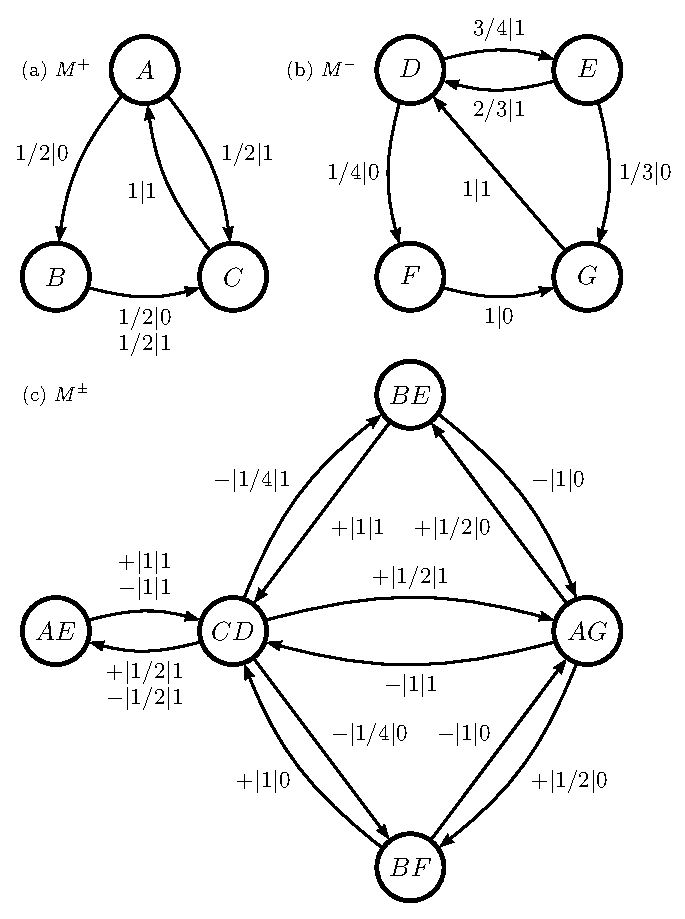
\includegraphics{RIP}}
\end{center}
\caption{
  Forward and reverse \eMs\ for the RIP: (a) $\FutureEM$ and (b) $\PastEM$.
  Edge labels $t|x$ give the transition probabilities
  $t = T_{\CausalState \CausalState^\prime}^{(x)}$.
  (c) The bidirectional machine $\BiEM$ for $p = q = 1/2$.
  Edge labels are prefixed with the scan direction $\{-,+\}$.
  }
\label{fig:RIP}
\end{figure}

The \eM\ information diagram of Fig.~\ref{fig:eMIDiagram} encapsulates all
of these results concisely by showing the key relationships between
information production ($H[\Future|\FutureCausalState]$ and 
$H[\Past|\PastCausalState]$), stored information 
($\FutureCmu$ and $\PastCmu$), and excess entropy 
(\mbox{$\EE = I[\Past;\Future]$}).  Analyzing the 4-variable information 
diagram revealed a parsimonious relationship among the four variables, 
depicted as differently shaded ellipses. $H[\Past]$ and $H[\Future]$
(two largest ellipses) are the entropies of the past and future, respectively,
which are the process's total information production. The information stored
in the predictive \eM\ $\FutureEM$ is its statistical complexity:
$\FutureCmu \equiv H[\FutureCausalState]$ (small ellipse on left); likewise
for $\PastEM$, $\PastCmu \equiv H(\PastCausalState)$ (small ellipse on right).
The excess entropy $\EE$ is the intersection of these sets; while the
statistical complexity $\BiCmu$ of the bidirectional machine $\BiEM$ is their
union; the crypticity $\PC$, their symmetric difference; and
their signed difference, the causal irreversibility $\CI$.

Consider an example that illustrates the typical process---cryptic
and causally irreversible. This is the Random Insertion Process (RIP) which
generates a random bit with bias $p$. If that bit is a $1$, then it outputs
another $1$. If the random bit is a $0$, however, it inserts another random
bit with bias $q$, followed by a $1$.

Its forward \eM, see Fig.~\ref{fig:RIP}(a), has three recurrent causal states
$\FutureCausalStateSet = \{ A, B, C \}$ and the transition matrices given there.
Figure~\ref{fig:RIP}(b) gives $\PastEM$ which has four recurrent causal states
$\PastCausalStateSet = \{ D, E, F, G \}$. We see that the \eMs\ are not the
same and so the RIP is causally irreversible. A direct calculation gives
$\Prob(\FutureCausalState) = \Prob(A,B,C) = (1, p, 1) / (p+2)$ and
$\Prob(\PastCausalState) = \Prob(D,E,F,G) = (1, 1-pq, pq, p) / (p+2)$. If
$p = q = 1/2$, for example, these give us $\FutureCmu \approx 1.5219$ bits,
$\PastCmu \approx 1.8464$ bits, and $\hmu = 3/5$ bits per measurement.
The causal irreversibility is $\CI \approx 0.3245$ bits.

Let's analyze its bidirectional machine; shown in Fig.~\ref{fig:RIP}(c) 
for $p = q = 1/2$. The interdependence between the forward
and reverse states is given by:
\vspace{-0.11in}
\begin{align*}
& \Pr(\FutureCausalState, \PastCausalState) = \frac{1}{(p+2)} 
 \times \bordermatrix{
   & D & E & F & G \cr
 A & 0 & 1-p & 0 & p \cr
 B & 0 & p(1-q) & pq & 0 \cr
 C & 1 & 0 & 0 & 0
} ~.
\end{align*}
By way of demonstrating the exact analysis now possible, $\EE$'s closed-form
expression for the RIP family is
\vspace{-0.09in}
\begin{align*}
\EE = \log_2 (p+2) - \frac{p \log_2 p }{p + 2} -
\frac{1-pq}{p + 2} H\left( \frac{1-p}{1-pq}\right) ~,
\end{align*}
where $H(\cdot)$ is the binary entropy function. The first two terms
on the RHS are $\FutureCmu$ and the last is
$H[\FutureCausalState|\PastCausalState]$.

Setting $p = q = 1/2$, one calculates that
$\Prob(\BiCausalState) = \Prob(AE,AG,BE,BF,CD) = \left(1/5,1/5,1/10,1/10,2/5\right)$.
This and the joint distribution give
$\BiCmu = H[\BiCausalState] \approx 2.1219$ bits,
but an $\EE = I[\FutureCausalState;\PastCausalState] \approx 1.2464$ bits.
That is,
the excess entropy (the apparent information) is substantially less than the
statistical complexities (stored information)---a rather cryptic process:
$\PC \approx 0.8755$ bits.

To close, the main results establish that when \mbox{$\PC > 0$} one cannot
simply use
sequence information directly to represent a process as storing $\EE$ bits
of information. We must instead store $\Cmu$ bits of information, building a
causal model of the hidden state information.
Why? Because typical processes encrypt their state information within their
observed behavior. More particularly, observed information can be arbitrarily
small ($\EE \approx 0$) compared to the stored information ($\Cmu$).

In deriving an explicit relationship between excess entropy and the \eM, the
framework puts prediction on an equal footing with modeling, allowing for
a direct comparison between them
\footnote{As noted for human language~\cite{Ebel94c,Debo08a},
$\EE$ and $C_\mu$ can diverge. Using methods
developed to analyze infinite \eMs~\cite{Crut01a,CompMechMerge}, we will
report extensions of the present results to such cases elsewhere.}.
Also, as we demonstrated with the RIP example,
it gives a way to develop closed-form expressions for $\EE$.  Finally and most
generally, it reveals an intimate connection between unpredictability,
irreversibility, crypticity, and information storage.

Practically, these results elucidate the difference between observed (mutual) 
information ($\EE$) and a process's stored information ($\Cmu$). Analyzing a 
process only in terms of mutual information misses an arbitrarily large 
amount of a process's structure. When this happens, one concludes that a 
process is more random than it is and that it has little structure, when 
neither is true.

Chris Ellison was partially supported by GAANN. The Network Dynamics Program
funded by Intel Corporation also partially supported this work.

\vspace{-0.21in}
\bibliography{ref,chaos}

\end{document}
